\documentclass[11pt]{article}
\usepackage[english]{babel}
\usepackage{amsmath, cite, mathtools, listings, textcomp, enumerate, fullpage}
\usepackage{graphicx, float, caption}

%\lstset{
%	language=R,
%	keywordstyle=\bfseries\ttfamily\color[rgb]{0,0,1},
%	identifierstyle=\ttfamily,
%	commentstyle=\color[rgb]{0.133,0.545,0.133},
%	stringstyle=\ttfamily\color[rgb]{0.627,0.126,0.941},
%	showstringspaces=false,
%	basicstyle=\tiny,
%	numberstyle=\scriptsize,
%	numbers=left,
%	stepnumber=1,
%	numbersep=10pt,
%	tabsize=2,
%	breaklines=true,
%	breakatwhitespace=false,
%	aboveskip={1.5\baselineskip},
%  columns=fixed,
%  upquote=true,
%  extendedchars=true,
%}

\title{Using RandomForests for Model Selection and Prediction on a Healthy Weight Survey for Young Children}
\author{Christopher Aden \and Christiana Drake \and Marilyn Townsend \and Mical Shilts}
\date{Sometime in June, 2015}

\begin{document}
\maketitle

\section*{Abstract}
We compare two statistical methods that identify the most predictive questions for various outcomes including predicting overweight status at a later time point. Head Start and WIC parents and their young children provided data: parent self-administered 43-item HealthyKids (HK) at 4 time points, nine 24-hour diet + activity recall logs, 3 blood samples and child anthropometrics collected at 3 time points. An importance plot determined the relative importance of each question by computing the average error when the particular question is omitted. Of the 43 behavioral items tested, 16 are selected for the final model. The chosen model has a similar classification rate as a stepwise regression procedure in looking at overweight status; it also selects the most predictive variables and provides a measure of their importance. The advantage of RandomForest is that it selected models reasonably supported by nutritional knowledge while avoiding problems faced by stepwise regression in fitting large models. RandomForest has potential for use in nutritional studies.

\section*{Introduction}
Classification is a common goal in nutrition, whether it be diagnosing an individual into non-diabetic or diabetic status, or predicting whether a child will become obese in the future. Common methods in the literature are logistic regression, discriminant analysis, and decision trees.

Logistic regression models look at the probability of being in a particular group using a linear combination of the predictors on the logit scale. Unlike more modern techniques, logistic regression allows one linear relationship of predictors, requiring that a single, global line be specified. The coefficients in a logistic regression model may be interpreted as the effect of the predictor on the log-odds ratio. For example, if we were modeling the probability that a child is overweight as a function of past BMI percentile, a coefficient of $.05$ would mean that for each 15-point increase in percentile, the odds of being overweight later in time would approximately double.

Classification and regression trees (CART) \cite{breiman1984classification} are a more flexible tool that partition the data into two categories, one predictor at a time, until the variability within a partition is homogeneous, relative to the other partitions. This process continues until we can no longer find a predictor that greatly reduces the heterogeneity. Like logistic regression, having more nodes decreases the in-sample misclassification, but also increases the complexity, making it harder to interpret. Both methods are also subject to ``over-fitting'' (observing a large out-of-sample error when the in-sample error is small). CART lacks the overall interpretation of logistic regression (coefficients as log-odds ratios), but computing predicted categories is straightforward and analogous to reading a flow chart. 

While there are many algorithms to build decision trees, we will outline the original CART algorithm proposed in \cite{breiman1984classification}. We assume there are $p$ predictor variables.

\begin{enumerate}[1.]
\item Find the predictor best at separating the responses into homogeneous splits. For classification, homogeneity is often measured with misclassification rate. For regression, a common metric is mean squared error. The best predictor will be the one that minimizes one of these metrics. The predictors are now split into two partitions, instead of the original one.
\item Starting at the top of the tree, select the predictor which minimizes the heterogeneity, but instead of splitting the whole predictor like last time, split only one of the partitions made in the first step. There are now three partitions.
\item Continue the process of finding predictors to split the space until some stopping criterion is reached. The default stopping mechanism used in the programming language \verb+R+'s implementation of CART \cite{Rpart} requires that a partition have at least 20 observations before a split, and that a split will not result in there being less than 7 observations in any one partition. Tree building stops at this point.
\item In each terminal node, classify to the most common category. If the objective is a regression, predict the mean of the responses of observations in the terminal node.
\end{enumerate}

This will usually produce trees that have too many splits, however. This makes the tree harder to interpret and hurts predictive performance on data that we didn't train the tree on. CART outlines a solution to this with a metod calling ``pruning'', by going back after growing a tree and finding smaller trees that manage to balance small tree size with a small error rate.

\subsection*{A Simulation Example}
The advantage of CART is that it allows for complicated interactions between predictors that would not be possible without adding many additional terms to a logistic regression. This makes it ideal in situations where the exact relationship of the predictors is unknown or difficult to specify.

We demonstrate the inability for logistic regression to classify as well as CART in problems where a linear logistic model does not work. We simulate data from two populations according to the following algorithm:

For $i=1, \dots, n_1$ negative samples (circles):
\begin{enumerate}
\item Sample $z_{1i}, z_{2i}$ independently from a standard normal, $N(0,1)$, distribution
\item Return covariates $x_{1i} = \cos(z_{1i}^2)$, and $x_{2i} = \left|z_{2i} \right| \cdot \sqrt{z_{1i}^2 + 1}$
\end{enumerate}

For $j = 1, \dots, n_2$ positive samples (crosses):
\begin{enumerate}
\item Sample $z_{1j}, z_{2j}$ independently from a standard normal, $N(0,1)$, distribution
\item Return covariates $x_{1j} = |z_{2j}*\sin(z_{1j})|$ and $x_{2j} = z_{1j} \cdot z_{2j}^2$
\end{enumerate}

The two variables are highly non-linear. While it is true that logistic regression can fit interactions between $x_1$ and $x_2$ and non-linear patterns, they must be explicitly accounted for. Logistic regression has trouble discriminating between the two groups because they overlap in a highly irregular way that is not explained well by simple linear relationships. With hypothesis testing, logistic regression would find significant relationships between both variables. This illustrates how it is possible to have a highly statistically significant model that is unable to predict well. As such, we cannot rely on hypothesis testing to show whether a model will be predictive.

\begin{figure}[H] \center
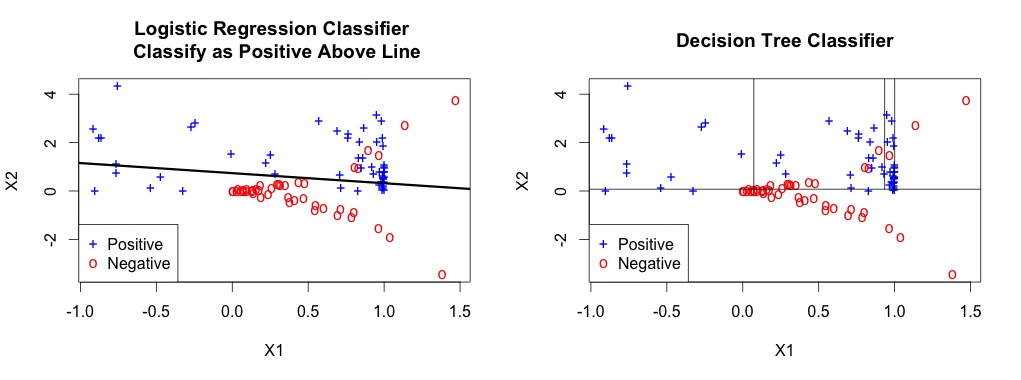
\includegraphics[scale=.35]{../Figures/Logit_vs_Tree.jpeg} 
\caption{A comparison of classification regions for logistic regression versus trees.}
\end{figure}

\begin{table}[H] \center
\caption{The hypothesis test for the logistic regression.}
\begin{tabular}{|c|c|c|c|c|} \hline
& Estimate & SE & $z$-value & $p$-value \\ \hline
(Intercept) & $-0.631$ & $0.103$ & $-6.155$ & $<0.00001$ \\ \hline
X1 & $0.357$ & $0.138$ & $2.592$ & $0.0096$ \\ \hline
X2 & $0.854$ & $0.080$ & $10.615$ & $<0.00001$ \\ \hline
\end{tabular}
\end{table}

CART are not without problems, however. They are very prone to over-fitting, that is, they tend to perform better on data used for estimating where to make splits in a classification problem. This hurts their predictive power, which is a task we want to carry out on data outside our sample. A more robust procedure would be to hold out some data each time and build a tree on the data that was not withheld, training afterwards on the hold-out. This leads us to RandomForests.

\section*{The RandomForest Algorithm}
RandomForests (RF) \cite{breiman2001random} is a statistical method that implements an improvement to the trees described above. RF is different from decision trees in that it combines information from many trees. This gives the forest robustness, as any over-fitting from any one single tree is averaged out. This means RF often has much higher accuracy than CART or logistic regression. However, because RF is based on an average of many trees, it cannot easily be interpreted or graphed--it is simply a tool for generating predictions and determining predictors.
In addition to the data, RandomForests takes two additioanl parameters: $B$, the number of trees to make, and $p$, the maximum number of predictors to use in each tree. Supposing that we had observed $n$ observations of $p$ predictors, $\mathbf{x_1}, \dots, \mathbf{x_n}$ (where $\mathbf{x_i} = (x_{i1}, x_{i2}, \dots, x_{ip})$) with $n$ corresponding responses $y_1, \dots y_n$. Then the algorithm goes as follows:
\begin{enumerate}
\item For each tree, $b = 1, \dots, B$:
	\begin{enumerate}
	\item Sample, with replacement, $n$ samples $\mathbf{x_{1}}, \dots, \mathbf{x_{n}}$, keeping only $p$ randomly selected predictors, and their corresponding responses $y_1, \dots, y_n$.
	\item Using this sampled data, create a tree $f_b$ using the CART algorithm described above, without pruning.
	\end{enumerate}
\item This procedure will generate $B$ trees. For a new observation $x'$, predict it's value by averaging over the output you would have acquired from each tree, i.e. $\hat{f}_{RF} (x') = \frac{1}{B} \sum_{i=1}^B f_i (x')$. This average output is the RandomForest estimator.
\end{enumerate}

The most alluring feature of RF, is the ability to fit models where there are a large number of predictors relative to sample size. Logistic regression will either not work, or work poorly in this case. RF averts this problem by fitting only a subset of the predictors at a time. RF gives us a novel method for determining which predictors are the most important for the outcome of interest. The variable importance plot works by computing the out-of-sample error for all trees, then omitting a particular predictor from that tree. The difference of these errors is then divided by the standard deviation of the differences over all trees. If a predictor has great predictive power, omitting it from a tree will greatly reduce the accuracy of the tree. Averaging results for all trees ensures that the predictor is not an artifact of one tree over-fitting a subset of data.

On our simulation task from before, RF completely dominates both logistic regression and trees. Below are the receiver operating characteristic (ROC) curves and the misclassification rates (in percent) for the three classifiers.

\begin{figure}[H] \center
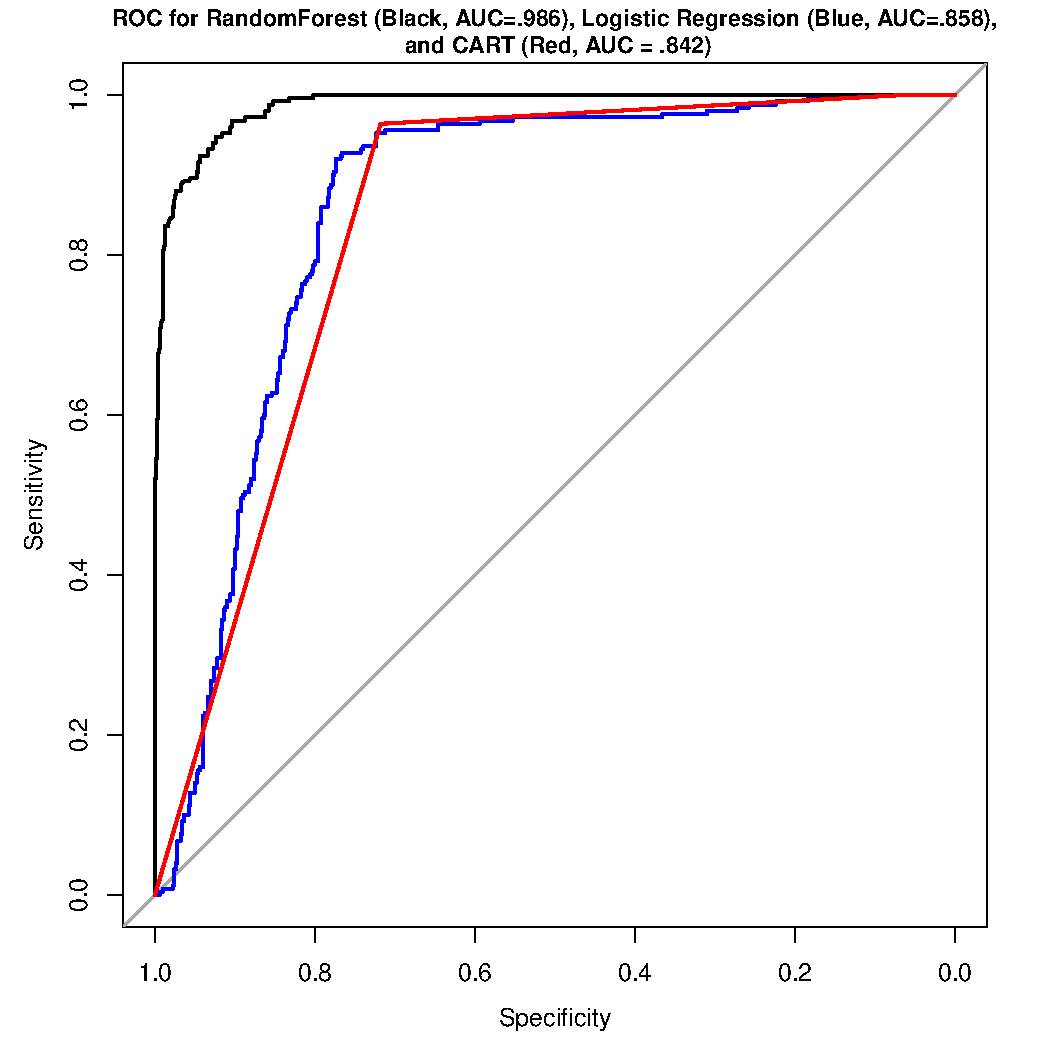
\includegraphics[scale=.5]{../Figures/ROC_LogitRF.pdf} 
\caption{ROC curves for logistic regression, CART, and RandomForests.}
\end{figure}

\begin{table}[H] \center
\caption{The hypothesis test for the logistic regression.}
\begin{tabular}{|c|c|c|} \hline
\textbf{Logistic} & Actually Positive & Actually Negative \\ \hline
Predicted Positive & $41$ & $13.6$ \\ \hline
Predicted Negative & $8.8$ & $36.5$ \\ \hline
\end{tabular}

\begin{tabular}{|c|c|c|} \hline
\textbf{CART} & Actually Positive & Actually Negative \\ \hline
Predicted Positive & $40.6$ & $5.3$ \\ \hline
Predicted Negative & $9.4$ & $44.7$ \\ \hline
\end{tabular}

\begin{tabular}{|c|c|c|} \hline
\textbf{RandomForests} & Actually Positive & Actually Negative \\ \hline
Predicted Positive & $46.3$ & $3.8$ \\ \hline
Predicted Negative & $3.7$ & $46.2$ \\ \hline
\end{tabular}
\end{table}

\section*{Application: Model Selection with RandomForests}
The Healthy Kids (HK) project looked at identifying the factors that make up healthy eating and activity habits in both parents and children. Head Start and WIC parents and their young children provided data: parent self-administered 43-item Healthy Kids (HK) at four time points, nine 24-hour diet and activity recall logs, three blood samples and child anthropometrics collected at three time points. 

Statistical modeling was employed to see if we could identify which children early-on would be overweight 24 months in the future, on the basis of current BMI percentile and the responses from their early questionnaires at baseline. The purpose was to see if we could predict from current BMI, eating habits, sleep, screen time, and physical activity whether a child would be overweight in the future.

Child-parent pairs ($n=90$) provided surveys and BMI measurements at the first survey administration (T3), first BMI measurement (T4) and the later BMI and survey administration (T13). Logistic regression was highly unstable trying to fit all survey questions ($p=44+1$ BMI Percentile), so forward stepwise regression was performed to reduce the number of predictors. Alternatively, we fit RandomForests on the same data set and used the variable importance plot to identify the most predictive questions.

\begin{figure}[H] \center
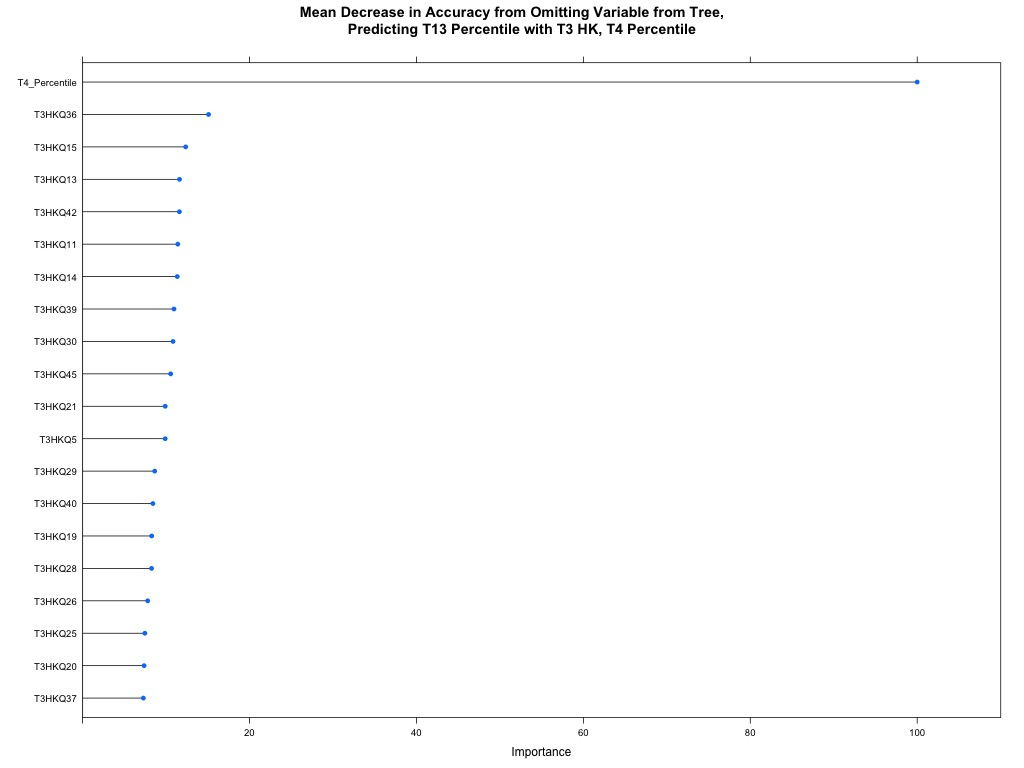
\includegraphics[scale=.4]{../Figures/HKVarImpPlot.jpeg} 
\caption{A Variable Importance Plot for the top 20 predictors with RF}
\end{figure}

\begin{table}[H] \center
\caption{Classification rates for the full logistic model, stepwise logistic model, and RandomForests}
\begin{tabular}{|c|c|c|} \hline
\textbf{Full Logistic} & Actually Positive & Actually Negative \\ \hline
Predicted Positive & $46.2$ & $16.5$ \\ \hline
Predicted Negative & $21.6$ & $15.6$ \\ \hline
\end{tabular}

\begin{tabular}{|c|c|c|} \hline
\textbf{Stepwise Logistic} & Actually Positive & Actually Negative \\ \hline
Predicted Positive & $59.5$ & $7.7$ \\ \hline
Predicted Negative & $8.2$ & $24.7$ \\ \hline
\end{tabular}

\begin{tabular}{|c|c|c|} \hline
\textbf{RandomForests} & Actually Positive & Actually Negative \\ \hline
Predicted Positive & $64$ & $10.6$ \\ \hline
Predicted Negative & $3.9$ & $21.6$ \\ \hline
\end{tabular}
\end{table}

Plotting the BMI Percentile as predicted by RandomForests against the predictors, we get an idea of the non-linearity of the predictors.
\textbf{(Plot here)}

\section*{Discussion and Conclusion}
The same framework used in classification problems can be used in regression problems with very minimal modification. Instead of needing to perform linear regression for continuous responses, and logistic regression in classification problems, RF can be used in a number of contexts, including continuous regression, classification, and survival analysis.

\nocite{*}
\bibliography{Publications}
\bibliographystyle{plain}
\end{document} 